\documentclass[a4paper,12pt]{article}

\usepackage[utf8]{inputenc}
\usepackage[spanish]{babel}
\usepackage{amsmath, amssymb}
\usepackage{graphicx}
\usepackage{float}
\usepackage{booktabs}
\usepackage{xcolor}
\usepackage{listings}
\usepackage{caption}
\usepackage{fancyhdr}
\usepackage{hyperref}
\usepackage{tikz}

\hypersetup{
    colorlinks=true,
    linkcolor=blue,
    urlcolor=blue,
    pdftitle={Práctica 2 - PIC32},
}

% === Definición de colores similares a Vivado ===
\definecolor{vivadoKeyword}{rgb}{0.6,0.0,0.6}
\definecolor{vivadoComment}{rgb}{0.0,0.5,0.0}
\definecolor{vivadoString}{rgb}{0.5,0.2,0.0}
\definecolor{vivadoBackground}{rgb}{0.97,0.97,0.97}

\lstdefinelanguage{VHDL}{
    morekeywords={library, use, entity, is, port, in, out, end, architecture, of, begin, signal, if, then, else, when, others, xor, and, or, not},
    sensitive=true,
    morecomment=[l]--,
    morestring=[b]",
}

\lstset{
    language=VHDL,
    backgroundcolor=\color{vivadoBackground},
    keywordstyle=\color{vivadoKeyword}\bfseries,
    commentstyle=\color{vivadoComment}\itshape,
    stringstyle=\color{vivadoString},
    basicstyle=\ttfamily\small,
    numbers=left,
    numberstyle=\tiny,
    numbersep=5pt,
    frame=single,
    breaklines=true,
    tabsize=2,
    captionpos=b
}

\title{Práctica N°2: Control de Motor DC con incremento de velocidad en PIC32 MAX32}
\date{}

\begin{document}
\maketitle
\tableofcontents
\newpage

\section{Objetivos}

\subsection{Objetivo general}
Implementar y analizar el control de velocidad de un motor de corriente continua (DC) utilizando la tarjeta \textbf{ChipKIT Max32} junto con el \textbf{Motor Shield}, aplicando la técnica de modulación por ancho de pulso (PWM) y un pulsador como interfaz de entrada para modificar dinámicamente el ciclo de trabajo.

\subsection{Objetivos específicos}
\begin{itemize}
    \item Comprender el principio de funcionamiento del \textbf{PWM} y su influencia en la velocidad de un motor DC.
    \item Configurar correctamente los pines de salida digital y PWM en la plataforma \textbf{ChipKIT Max32}.
    \item Implementar un programa que incremente el valor del ciclo de trabajo del PWM mediante un \textbf{pulsador} conectado a una entrada digital.
    \item Analizar el comportamiento del motor frente a los cambios en el ciclo de trabajo y observar la variación de la velocidad.
    
\end{itemize}

\section{Descripción del código}

A continuación se presenta el código fuente implementado para controlar un motor de corriente continua mediante la tarjeta \textbf{ChipKIT Max32} y el \textbf{Motor Shield}. El programa permite variar el ciclo de trabajo del PWM utilizando un único pulsador conectado a una entrada digital configurada con resistencia \textit{pull-up} interna.

\begin{lstlisting}[language=C, caption={Código fuente para el control de un motor DC con el ChipKIT Max32 y Motor Shield}, label={lst:pic32_motor_pwm}]
 // Prueba simple para motor con ChipKIT Max32 + Motor Shield
 // PWM -> pin 3 (RD0 / OC1)
 // DIR -> pin 4 (RF1)
 // BTN -> pin 7 (a GND, use INPUT_PULLUP)  <-- único botón

 const int PWM_PIN   = 3;   // RD0 / OC1
 const int DIR_PIN   = 4;   // RF1
 const int BTN       = 78;  // botón (a GND)

 int duty = 0;              // 0..255 (valor inicial)
 const int STEP = 25;       // incremento por pulsación
 const int DUTY_MIN = 0;
 const int DUTY_MAX = 255;

 int lastButtonState = HIGH; // estado anterior del botón (INPUT_PULLUP: idle = HIGH)

 void setup() {
   pinMode(PWM_PIN, OUTPUT);
   pinMode(DIR_PIN, OUTPUT);
   pinMode(BTN, INPUT_PULLUP);

   // Estado inicial
   digitalWrite(DIR_PIN, LOW);
   analogWrite(PWM_PIN, duty);
 }

 void loop() {
   int current = digitalRead(BTN);

   // Detección de flanco: HIGH -> LOW significa "pulsado"
   if (lastButtonState == HIGH && current == LOW) {
     duty += STEP;
     if (duty > DUTY_MAX) duty = DUTY_MIN; // si supera el máximo, reinicia
     analogWrite(PWM_PIN, duty);
   }

   lastButtonState = current;
   delay(100); // pequeño retardo para aliviar CPU (no es debounce)
 }
\end{lstlisting}

\subsection{Explicación paso a paso}

\begin{enumerate}
    \item \textbf{Definición de pines:}  
    Se definen tres pines principales:
    \begin{itemize}
        \item \texttt{PWM\_PIN = 3}: salida de modulación por ancho de pulso (PWM) correspondiente al pin RD0/OC1 del PIC32.  
        \item \texttt{DIR\_PIN = 4}: controla la dirección del giro del motor mediante el pin RF1.  
        \item \texttt{BTN = 78}: entrada digital conectada a un pulsador. Se utiliza la resistencia interna \texttt{INPUT\_PULLUP}, por lo que el estado lógico será \texttt{HIGH} en reposo y \texttt{LOW} al presionar.
    \end{itemize}

    \item \textbf{Variables de control:}  
    Se define \texttt{duty} como la variable que determina el ciclo de trabajo del PWM (rango de 0 a 255).  
    La constante \texttt{STEP = 25} indica el incremento de velocidad en cada pulsación del botón.  
    Cuando el valor supera \texttt{255}, se reinicia a cero.

    \item \textbf{Configuración inicial (\texttt{setup()})}:  
    Los pines se configuran como salidas o entradas según su función.  
    Luego se establece un estado inicial: dirección baja (\texttt{LOW}) y ciclo de trabajo inicial de 0, manteniendo el motor detenido al inicio.

    \item \textbf{Bucle principal (\texttt{loop()})}:  
    En cada iteración se lee el estado actual del botón (\texttt{digitalRead(BTN)}).  
    Se compara el estado anterior (\texttt{lastButtonState}) con el actual para detectar un \textbf{flanco descendente} (transición de \texttt{HIGH} a \texttt{LOW}), que representa una pulsación.

    \item \textbf{Ajuste del PWM:}  
    Cada vez que se detecta una pulsación, se incrementa el ciclo de trabajo en \texttt{STEP} unidades.  
    Si el valor supera el máximo (\texttt{255}), se reinicia a cero, permitiendo un ciclo continuo de aumento.

    \item \textbf{Actualización del motor:}  
    El nuevo valor de \texttt{duty} se aplica con \texttt{analogWrite(PWM\_PIN, duty)}, modificando la velocidad del motor.

    \item \textbf{Pequeño retardo:}  
    Se agrega un retardo de 100\,ms mediante \texttt{delay(100)} para evitar lecturas excesivas y reducir la carga del procesador.  
    Este retardo no cumple la función de \textit{debounce}, pero mejora la estabilidad básica del programa.
\end{enumerate}

\section{Resultados}

En la Figura~\ref{fig:resultado_motor} se muestra el resultado del funcionamiento del sistema implementado con la tarjeta \textbf{ChipKIT Max32} y el \textbf{Motor Shield}.  
Se observa el motor de corriente continua en operación, cuya velocidad varía conforme se presiona el pulsador, modificando el ciclo de trabajo del PWM generado por el microcontrolador.

\begin{figure}[H]
    \centering
    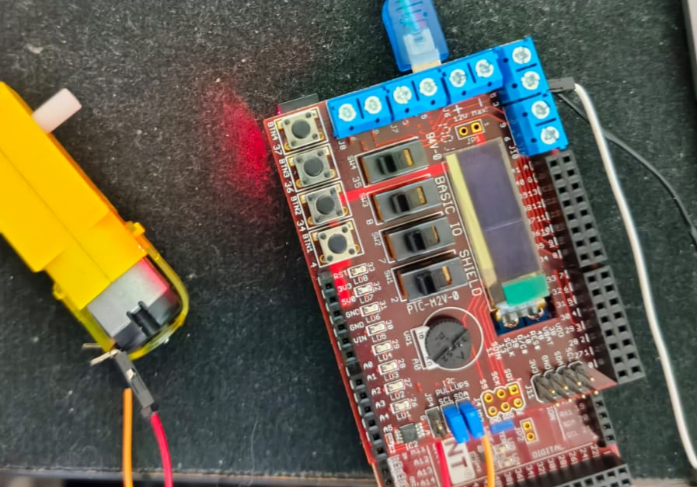
\includegraphics[width=0.8\textwidth]{funcion.png}
    \caption{Funcionamiento del motor DC controlado por PWM usando la tarjeta ChipKIT Max32 y el Motor Shield.}
    \label{fig:resultado_motor}
\end{figure}


\end{document}
